\begin{flushright} {\tiny {\color{gray} python\_codes/fieldstone\_121/text.tex}} \end{flushright}

%\lstinputlisting[language=bash,basicstyle=\small]{python_codes/fieldstone_01/keywords}

\begin{center}

\fbox{\textbf{\huge \color{teal} P}}
Code at \url{https://github.com/cedrict/fieldstone/tree/master/python_codes/fieldstone_121}
\end{center}

\par\noindent\rule{\textwidth}{0.4pt}

%%%%%%%%%%%%%%%%%%%%%%%%%%%%%%%%%%%%%%%%%%%%%%%%%%%%%%%%%%%%%%%%%%%%%%%%%%%%%%%%%%%%%%%%%%%%%%%%

The domain is a 2D Cartesian box of size $L_x \times L_y$ with 
$L_x=200~\si{\km}$ and $L_y=100~\si{\km}$.
The isothermal incompressible Stokes equations are solved on a mesh 
of $nelx\times nely$ $Q_2\times Q_1$ elements (same as \aspect).
 

It contains a single fluid characterised by the dislocation creep 
effective viscosity of \textcite{gatt20} (2020) and \textcite{gath21} (2021):
\[
\eta_{disl}(\dot{\varepsilon}_e,T)  = \frac{A_0}{2\dot{\varepsilon}_e}\left[ 
1 + \tanh\left( A_1 ( \log_{10}   \dot{\varepsilon}_e - A_2 )  \right)
\right]
\]
with 
\begin{align}
A_0(T) &= a_0 + b_0 T \nn\\ 
A_1(T) &= a_1 + b_1 T \nn\\ 
A_2(T) &= a_2 + b_2 T +c_2T^2 \nn
\end{align}
and
\begin{align}
a_0 &= 4.4\cdot 10^8 \nn\\
b_0 &= -5.26\cdot 10^4 \nn\\
a_1 &= 2.11\cdot 10^{-2} \nn\\
b_1 &= 1.74\cdot 10^{-4} \nn\\
a_2 &= -41.8 \nn\\
b_2 &= 4.21\cdot 10^{-2} \nn\\
c_2 &= -1.14\cdot 10^{-5} \nn
\end{align}

The setup is similar to the one in \textcite{gupm14} (2014) although the formulation here is purely 
Eulerian and will rely on periodic boundary conditions when large shear values are used.
Boundary conditions are $\vec{\upnu}=(+u_0,0)$ on the top, $\vec{\upnu}=(-u_0,0)$ on the 
bottom, and $v=0$ on the left and right boundaries. We thereby obtain a flow 
that is parallel to the $x$-axis. $u_0$ is set to $1~\si{\cm\per\year}$.

The rheology is nonlinear so Picard nonlinear iterations are implemented. These stop
when the difference between two consecutively obtained velocity fields falls below
a given tolerance $tol=10^{-3}$. 

The temperature field is set to a constant value $T_0$ throughout the domain.

If no thermal or mechanical inhomogeneity is implemented, this setup results in 
a velocity field $\vec{\upnu}=(u,v)$ that is such that $v(x,y)=0$, and 
$u(x,y)=2u_0 (y-L_y/2)/L_y$, with $\dot{\varepsilon}_{xx}=\dot{\varepsilon}_{yy}=0$ 
and $\dot{\varepsilon}_{xy}=u_0/L_y$. 

\begin{center}
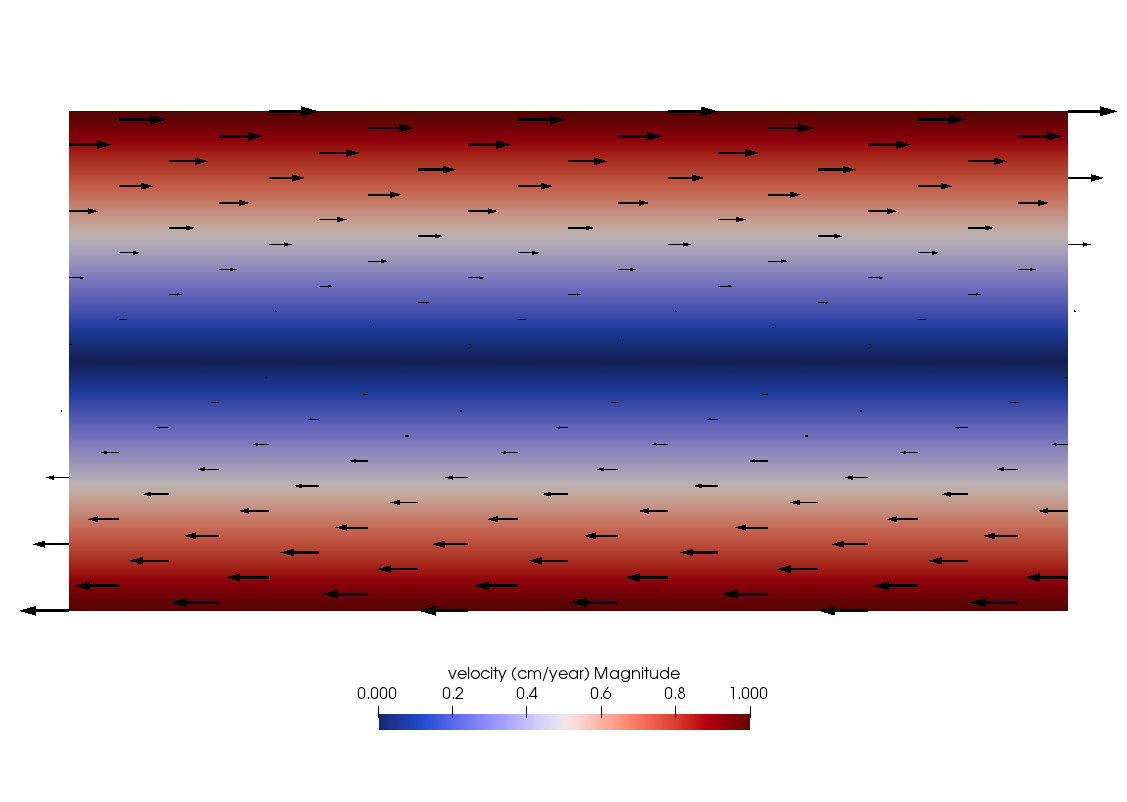
\includegraphics[width=7cm]{python_codes/fieldstone_121/results/vel}
\end{center}

We therefore need a form of weak seed/zone to localise the deformation and 
initiate the strain weakening process.

I will soon implement a passive set of particles on which strain can be accumulated so as 
to allow for strain weakening. What form should the strain weakening take?


\newpage

The deformation mechanism equations are from \textcite{gupr14} (2014):
\[
\dot\varepsilon = \dot\varepsilon_{dsl} + \dot\varepsilon_{dif} + \dot\varepsilon_{gbs} + \dot\varepsilon_{exp} 
\]
with
\begin{eqnarray}
\dot\varepsilon_{dsl} &=& A_{dsl} \exp \left(-\frac{Q_{dsl}}{RT} \right)  \tau^{n_{dsl}}  \\
\dot\varepsilon_{dif} &=& A_{dif} \exp    \\
\dot\varepsilon_{gbs} &=& A_{gbs} \exp    \\
\dot\varepsilon_{exp} &=& A_{exp} \exp    
\end{eqnarray}





